\reading{IM-3}{Alpha (and the Low-Risk Anomaly)}{STRIKE FIRST}{5}

\srcnote{Andrew Ang, \textit{Asset Management: A Systematic Approach to Factor
Investing} (New York, NY: Oxford University Press, 2014), Chapter 10.
Printed as Chapter 3 in the GARP source volume.}

\begin{imkeybox}[title={The nine objectives in this reading}]
\begin{enumerate}[label=\textbf{\alph*.}]
\item Describe and evaluate the low-risk anomaly of asset returns.
\item Define and calculate alpha, tracking error, the information ratio, and the Sharpe ratio.
\item Explain the impact of benchmark choice on alpha and describe characteristics of an effective benchmark to measure alpha.
\item Describe Grinold's fundamental law of active management, including its assumptions and limitations, and calculate the maximum attainable information ratio using this law.
\item Apply a factor regression to construct a benchmark with multiple factors, measure a portfolio's sensitivity to those factors, and measure alpha against that benchmark.
\item Explain how to use style analysis to handle time-varying factor exposures.
\item Describe issues that arise when measuring alphas for nonlinear strategies.
\item Compare the volatility anomaly and the beta anomaly and analyze evidence of each anomaly.
\item Describe potential explanations for the risk anomaly.
\end{enumerate}
\end{imkeybox}

\begin{imtrapbox}[breakable=false,title={Two layers, two numbering schemes}]
This reading is covered twice in the source notes. The crash layer labels it
\emph{Reading 85}, which is correct under GARP's global sequential numbering.
The lecture layer labels the same material \emph{LO 80.a, 80.g, 80.h, 80.i} ---
an off-by-five run pointing at LTR-15, an unrelated liquidity reading. Both
layers are merged below under the spine's letters.
\end{imtrapbox}

% ------------------------------------------------------------------
\lo{IM-3 a}{Describe and evaluate the low-risk anomaly of asset returns.}

The capital asset pricing model from traditional finance states that there should
be a positive relationship between risk and return: higher risk, as measured by
beta, should have a higher return.

\begin{imdefbox}[title={The low-risk anomaly}]
A phenomenon that challenges one of the fundamental principles of traditional
finance --- the positive relationship between risk and return as defined by the
CAPM. \term{This anomaly finds that firms with lower betas and lower volatility
have higher returns over time.}
\end{imdefbox}

\figwrap{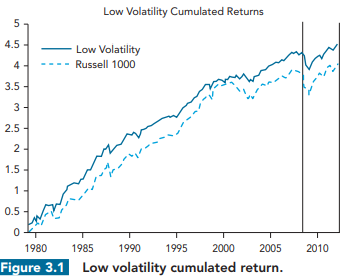
\includegraphics[width=8.4cm]{fig/p14-004.png}}%
{Cumulated returns on a low-volatility strategy against the Russell 1000, 1980
to 2012, reproduced from the source notes (GARP Figure 3.1). The vertical line
marks the point where the simulation ends and live performance begins. This is a
real return series and is embedded rather than redrawn. The low-volatility line
finishes above the index --- which under the CAPM it should not, because it is
the \emph{less} risky of the two.}

The ``risk anomaly'' suggests that low-risk stocks yield high returns, providing
a source of alpha compared to traditional benchmarks and other dynamic factors.

% ------------------------------------------------------------------
\lo{IM-3 b}{Define and calculate alpha, tracking error, the information ratio, and the Sharpe ratio.}

\begin{enumerate}
\item \term{Alpha ($\alpha$)} measures average excess return compared to a
benchmark (e.g.\ the S\&P 500). Excess return is the difference between the
asset's return and the benchmark return.
\item \term{Tracking error} is the standard deviation of excess returns. It shows
how much your returns deviate from the benchmark. Higher tracking error means
your returns stray further from the benchmark, which is more risk.
\item \term{Information ratio (IR)} is alpha divided by tracking error ---
alpha adjusted for risk. Higher is better.
\item \term{Sharpe ratio} is alpha divided by the standard deviation of the
asset's return, when the risk-free rate is the benchmark. It measures
risk-adjusted performance. Higher is better.
\end{enumerate}

\begin{imfmlbox}
\[ \text{IR} = \frac{\alpha}{\text{tracking error}}
   \qquad\qquad
   \text{SR} = \frac{\alpha}{\sigma} \;\;\text{(benchmark} = r_f) \]
\vk{the two ratios share a numerator and differ only in the denominator. The
information ratio divides by the standard deviation of \emph{excess} returns; the
Sharpe ratio divides by the standard deviation of the \emph{asset's own} returns.}
\end{imfmlbox}

\begin{imtrapbox}[breakable=false,title={The denominator is the discriminator}]
Alpha, IR and SR all sit on the same numerator. Every one of the three changes
when the benchmark changes, because the benchmark defines what counts as excess.
A distractor that alters the numerator while claiming to distinguish IR from SR
has attacked the wrong term.
\end{imtrapbox}

% ------------------------------------------------------------------
\lo{IM-3 c}{Explain the impact of benchmark choice on alpha and describe characteristics of an effective benchmark to measure alpha.}

A benchmark is very important for investment comparisons. \term{If the benchmark
is riskier than the investment in question, then both the alpha and the
information ratio will be too low.}

\subsection{The ideal benchmark}

\begin{enumerate}
\item \term{Well defined.} The identities and weights of securities or factor
exposures constituting the benchmark are clearly defined. The Russell 1000 is
verifiable and free of ambiguity about its contents.
\item \term{Tradeable.} Alpha must be measured against a tradable benchmark. The
benchmark should be a realistic, low-cost alternative for the asset owner. The
Russell 1000 is a natural passive benchmark because low-cost mutual fund and ETF
versions are available.
\item \term{Replicable.} The benchmark is consistent with the manager's
investment style or area of expertise.
\item \term{Adjusted for risk.} Failing to adjust the benchmark for risk can make
a huge difference in the alpha; a sound benchmark should be reflective of the
manager's current investment opinions.
\end{enumerate}

% ------------------------------------------------------------------
\lo{IM-3 d}{Describe Grinold's fundamental law of active management, including its assumptions and limitations, and calculate the maximum attainable information ratio using this law.}

A portfolio manager creates alpha relative to a benchmark by making bets that
deviate from that benchmark. Grinold's fundamental law of active management
states that the maximum information ratio attainable is given by:

\begin{imfmlbox}
\[ \text{IR} \;=\; \text{IC} \times \sqrt{\text{BR}} \]
\vk{IR is the information ratio; IC is the \term{information coefficient}, the
correlation of the manager's forecast with the actual returns --- how good the
forecasts are; and BR is the \term{breadth} of the strategy, how many bets are
taken. Breadth is the number of securities that can be traded and how frequently
they can be traded.}
\end{imfmlbox}

\begin{imtrapbox}[breakable=false,title={A dropped square root}]
The source notes print this law as $\text{IR} \approx \text{IC} \times
\text{BR}$, without the radical. The radical is the entire content of the law.
With 400 bets a year and an IC of $0.025$, the correct law gives
$0.025 \times \sqrt{400} = 0.50$; the notes' version gives
$0.025 \times 400 = 10.0$, an information ratio twenty times larger than any
manager has ever achieved. Restored from GARP Equation 3.5.
\end{imtrapbox}

Grinold and Kahn summarise it as: \term{it is important to play often} (high
breadth) \term{and to play well} (high IC).

\gapbadge
\srcnote{The notes state the law but work no example with it, so the square root
never has to do anything. The two cases below are GARP's own (Chapter 3), and
they are the reason the radical matters.}

\begin{imexbox}[title={Two managers, the same information ratio}]
A stock market timer trading just the aggregate market has \term{narrow breadth}:
there are few assets, sometimes just stocks and bonds. Making only four bets a
year, her bets have to be very accurate.
\[ \text{IR} = 0.25 \times \sqrt{4} = 0.25 \times 2 = 0.50 \]
A stock selector running value, size or momentum has \term{great breadth},
because hundreds of stocks can be traded. Making four hundred independent bets a
year:
\[ \text{IR} = 0.025 \times \sqrt{400} = 0.025 \times 20 = 0.50 \]
Both reach an information ratio of $0.50$. The timer needs an IC of $0.25$; the
selector needs an IC of $0.025$, a tenth as much.
\end{imexbox}

\figwrap{%
\begin{tikzpicture}
\begin{axis}[frmaxis,
  width=11.4cm, height=5.6cm,
  xmode=log, log basis x=10,
  xmin=2, xmax=900, ymin=0, ymax=0.45,
  xlabel={breadth BR --- number of independent bets per year (log scale)},
  ylabel={IC required},
  xtick={4,10,40,100,400}, xticklabels={4,10,40,100,400},
]
\addplot[FRMNavy, very thick, smooth, domain=2:900, samples=120] {0.5/sqrt(x)};
\addplot[only marks, mark=*, mark size=2.2pt, FRMRed] coordinates {(4,0.25)};
\addplot[only marks, mark=*, mark size=2.2pt, FRMGreen] coordinates {(400,0.025)};
\node[font=\scriptsize\sffamily, fill=white, inner sep=1.5pt, anchor=west,
      text=FRMRed] at (axis cs:5.2,0.27) {market timer: 4 bets, IC $=0.25$};
\node[font=\scriptsize\sffamily, fill=white, inner sep=1.5pt, anchor=east,
      text=FRMGreen] at (axis cs:330,0.075) {stock selector: 400 bets, IC $=0.025$};
\end{axis}
\end{tikzpicture}}%
{The skill a manager needs, as a function of how often she can play. The curve is
$\text{IC} = \text{IR}/\sqrt{\text{BR}}$ for a fixed information ratio of $0.50$.
Both marked managers sit on the same curve and earn the same information ratio.
Note the log scale: multiplying breadth by one hundred divides the required skill
by ten, not by one hundred. That is what the square root does, and it is why a
low-edge, high-turnover strategy can compete with a high-conviction one.}

\subsection{Assumptions and limitations}

\begin{itemize}
\item \term{Assumptions.} It ignores transactions costs, trading restrictions and
other real-world considerations --- which is why the resulting information ratio
is the \emph{maximum attainable}. A crucial assumption is that the forecasts are
independent of each other.
\item \term{Limitations.} The law is derived under mean-variance utility, so all
the shortcomings of mean-variance utility apply. In particular it ignores
downside risk and other higher moment risk, while assuming that all information
is used optimally.
\item In financial practice, a jump in asset prices chosen by asset managers often
causes the decline of IC, which is a reason why some mutual funds are willing to
block new investors and assets once they have met their internal requirements.
\end{itemize}

% ------------------------------------------------------------------
\lo{IM-3 e}{Apply a factor regression to construct a benchmark with multiple factors, measure a portfolio's sensitivity to those factors, and measure alpha against that benchmark.}

The traditional capital asset pricing model only accounts for co-movement with a
market index. Multifactor models, like the Fama and French three-factor model,
add other explanatory factors in an attempt to better predict the alpha for an
asset.

\subsection{Factor regressions}

First we verify alpha, or excess returns, via the CAPM benchmark:

\begin{imfmlbox}
\[ R_{i,t} - R_F = \alpha + \beta\,(R_M - R_F) + \varepsilon_{i,t} \]
\end{imfmlbox}

Then the Fama-French model adds two other factors:

\begin{imfmlbox}
\[ R_i - R_F = \alpha + \beta_{i,\text{MKT}}(R_M - R_F)
   + \beta_{i,\text{SMB}}(\text{SMB}) + \beta_{i,\text{HML}}(\text{HML}) \]
\vk{a positive $s$ (the SMB loading) means the asset moves with small stocks; a
negative $s$ means it moves with large stocks. A positive $h$ (the HML loading)
indicates a value orientation; a negative $h$ indicates growth. The market itself
is neither small nor big and neither value nor growth, so it has zero $s$ and
zero $h$.}
\end{imfmlbox}

\subsection{The worked case: Berkshire Hathaway}

\renewcommand{\arraystretch}{1.25}
\noindent\begin{tabularx}{\textwidth}{@{}p{4.2cm}rrrX@{}}
\toprule
& \textbf{\sffamily\small CAPM} & \textbf{\sffamily\small Fama-French} & \textbf{\sffamily\small \,$+$ momentum} & \\
\midrule
Alpha (per month) & 0.72\% & 0.65\% & 0.68\% & \\
Market loading & 0.51 & 0.67 & 0.66 & \\
SMB loading & --- & $-0.50$ & $-0.50$ & \\
HML loading & --- & 0.38 & 0.36 & \\
UMD loading & --- & --- & $-0.04$ & \\
Adjusted $R^2$ & 14\% & 27\% & 27\% & \\
\bottomrule
\end{tabularx}
\renewcommand{\arraystretch}{1}
\figcap{Buffett measured against three benchmarks. Controlling for size and value
knocks the alpha from 0.72\% to 0.65\% per month --- nearly 1\% a year --- and
lifts the adjusted $R^2$ from 14\% to 27\%. The negative SMB loading and positive
HML loading say the same thing an ordinary reader of Berkshire's letters already
knew: it is a large, value investor. Adding momentum changes nothing: the UMD
loading is $-0.04$ and insignificant, the $R^2$ does not move, and the alpha
actually rises slightly.}

The factor loadings translate directly into a benchmark portfolio. The benchmark
implied by the Fama-French estimates is:

\begin{imdefbox}[title={The mimicking portfolio, per \$1 of capital}]
\begin{tabbing}
\hspace{3.6cm}\=\kill
$(1-0.67) = \$0.33$ \> in T-bills \\
$+\ \$0.67$ \> in the market portfolio \\
$-\ \$0.50$ \> in small caps \qquad $+\ \$0.50$ in large caps \\
$+\ \$0.38$ \> in value stocks \qquad $-\ \$0.38$ in growth stocks
\end{tabbing}
\vspace{2pt}
In addition to this benchmark, Buffett is generating $+0.65\%$ alpha per month.
\end{imdefbox}

The cash and market weights sum to \$1, and the two long-short overlays each net
to zero: $-0.50 + 0.50 = 0$ for size and $+0.38 - 0.38 = 0$ for value. \term{It
still represents \$1 of capital allocated between factor portfolios.} Every time
we run a factor regression, we are assuming that we can create a factor benchmark
portfolio.

\gapbadge
\srcnote{The source notes reach ``Then, adding momentum to the above model'' and
stop; the four-factor equation and its result are absent. Written below from GARP
Chapter 3, Equation 3.11.}

\begin{imfmlbox}
\[ r_{it} - r_{ft} = \alpha + \beta(r_{mt}-r_{ft}) + s\,\text{SMB}_t
   + h\,\text{HML}_t + u\,\text{UMD}_t + \varepsilon_{it} \]
\vk{UMD is the momentum factor, long stocks that have gone \emph{up} and short
stocks that have gone \emph{down}. First done by Carhart (1997).}
\end{imfmlbox}

The four-factor mimicking portfolio is the three-factor one with $\$0.34$ in
T-bills, $\$0.66$ in the market, the same $\mp\$0.50$ size overlay, a
$\pm\$0.36$ value overlay, and $-\$0.04$ in past winners against $+\$0.04$ in
past losers.

\begin{imtrapbox}[breakable=false,title={An arithmetic slip in the source book}]
GARP prints the four-factor cash weight as ``$(1 - 0.66) = \$0.37$ in T-bills.''
The expression is right and the figure is not: $1 - 0.66 = 0.34$. The weight
shown above is $\$0.34$, which is what the stated market loading of $0.66$
requires if the portfolio is to represent \$1 of capital. Flagged rather than
silently adopted.
\end{imtrapbox}

% ------------------------------------------------------------------
\lo{IM-3 f}{Explain how to use style analysis to handle time-varying factor exposures.}

\subsection{Limitations of a regular multifactor regression}

\begin{enumerate}[label=\alph*)]
\item Uses static factors (betas) that don't change over time.
\item Relies on factors (SMB, HML) that aren't directly tradable.
\end{enumerate}

\subsection{Style analysis: a more flexible approach}

\begin{enumerate}[label=\alph*)]
\item Addresses time-varying factor exposures by allowing betas to change.
\item Uses tradable assets (e.g.\ ETFs) to represent factors.
\end{enumerate}

\begin{imkeybox}
Style analysis fixes both limitations at once, and that pairing is the point:
betas become dynamic \emph{and} the factors become things you can actually buy.
\end{imkeybox}

% ------------------------------------------------------------------
\lo{IM-3 g}{Describe issues that arise when measuring alphas for nonlinear strategies.}

When measuring alphas for nonlinear strategies, several issues arise.

\begin{itemize}
\item \term{Linear framework of alpha calculation.} Alpha is traditionally
computed using linear regression techniques. Nonlinear strategies, such as
uncovered long put options, have nonlinear payoff profiles (like an L-shape),
which can falsely yield a positive alpha when using linear methods. Strategies
with quadratic or option-like payoff structures, like $\max(R_t, 0)$, create
challenges in measuring alpha accurately because these payoffs do not align well
with linear regression-based alpha calculations.
\item \term{Non-normal distribution.} The distribution of returns for nonlinear
strategies often deviates from a normal distribution. This departure from
normality can affect the reliability of alpha calculations, as alpha assumes a
normally distributed return distribution.
\item \term{Negative skewness.} Certain nonlinear strategies exhibit negative
skewness in their return distribution, meaning a higher potential for losses on
the left tail. Alpha calculations typically do not account for skewness.
\end{itemize}

These issues are particularly relevant to hedge funds that employ nonlinear
strategies like merger arbitrage, pairs trading, and convertible bond arbitrage,
where the payoff structures are not linear.

\figwrap{%
\begin{tikzpicture}
\begin{axis}[frmaxis,
  width=11.4cm, height=5.8cm,
  xmin=-0.16, xmax=0.66, ymin=-2.0, ymax=1.5,
  xlabel={market excess return}, ylabel={strategy return},
  legend style={font=\scriptsize\sffamily, draw=FRMRule, fill=white,
    at={(0.5,-0.26)}, anchor=north, legend columns=-1, column sep=10pt},
]
\addplot[only marks, mark=*, mark size=1.5pt, FRMNavy] coordinates {
  (-0.10,1.10) (-0.05,0.68) (-0.04,0.62) (-0.03,0.52) (-0.02,0.45)
  (-0.005,0.31) (0.005,0.14) (0.06,-0.22) (0.08,-0.52) (0.11,-0.80)
  (0.115,-0.86) (0.125,-0.95) (0.19,-0.96) (0.30,-0.95) (0.32,-0.95)
  (0.39,-0.94) (0.49,-0.93) (0.59,-0.92)};
\addlegendentry{strategy payoffs}
\addplot[FRMRed, very thick, domain=-0.16:0.66, samples=2] {0.1182 - 2.8887*x};
\addlegendentry{fitted CAPM line}
\draw[black!45, thin] (axis cs:-0.16,0) -- (axis cs:0.66,0);
\node[font=\scriptsize\sffamily, fill=white, inner sep=1.5pt, anchor=west,
      text=FRMRed] (al) at (axis cs:0.08,0.95) {fitted $\alpha = +0.118$};
\draw[-{Stealth[length=4pt]}, FRMRed, thin] (al.west) -- (axis cs:-0.005,0.16);
\end{axis}
\end{tikzpicture}}%
{The alpha illusion, redrawn and refitted. The payoffs are L-shaped: the strategy
makes money only when the market falls and is pinned near $-0.95$ for every
positive market return. Fitting a straight line through that shape produces a
\emph{positive} intercept --- an alpha of $+0.118$ on this reconstruction, and
$+0.074$ on GARP's own Figure 3.7 --- even though the strategy loses money in
almost every state that actually occurs. The alpha is an artefact of forcing a
line through a kink, not a reward for skill.}

% ------------------------------------------------------------------
\lo{IM-3 h}{Compare the volatility anomaly and the beta anomaly and analyze evidence of each anomaly.}

\subsection{The volatility anomaly}

\begin{itemize}
\item Haugen and Heins (1975) observed a long-term trend where stock portfolios
with lower variance in monthly returns tended to yield greater average returns.
\item Ang, Hodrick, Xing and Zhang (2006) covered September 1963 to December 2011,
organised data into quintiles and controlled for leverage, volume, bid-ask
spreads, analyst forecasts and momentum.
\item Sorting on idiosyncratic volatility, average returns are above 10\% for the
first three quintiles, fall to \term{6.8\%} for quintile 4, and then plummet to
\term{0.1\%} for the highest-volatility stocks. Raw Sharpe ratios decline
monotonically from \term{0.8 to 0.0}.
\end{itemize}

\begin{imtrapbox}[breakable=false,title={What declines, and what does not}]
The source notes say that ``as standard deviation increased, both average returns
and Sharpe ratios decreased.'' The data do not say that. Average returns are
\emph{above 10\% for the first three quintiles} and only collapse at quintiles 4
and 5. The quantity that declines monotonically is the \term{Sharpe ratio}, from
0.8 to 0.0. Corrected from GARP Chapter 3, Figure 3.8.
\end{imtrapbox}

\subsection{The beta anomaly}

Sorting instead on beta, the picture is different in a way that is the whole
examinable point:

\begin{imkeybox}
\term{The beta anomaly is not that stocks with high betas have low returns ---
they don't.} Average returns across the beta quintiles are approximately flat,
around 15\% for the first four quintiles and slightly lower at 12.7\% for
quintile 5. Stocks with high betas have high \emph{volatilities}. That is what
causes the Sharpe ratios of high-beta stocks to be lower, dropping from 0.9 to
0.4.
\end{imkeybox}

\figwrap{%
\begin{tikzpicture}[
  hd/.style={draw=FRMNavy,fill=FRMNavy,rounded corners=1pt,inner sep=4pt,
             font=\scriptsize\sffamily\bfseries,text=white,align=center,
             text width=42mm},
  bx/.style={draw=FRMRule,fill=white,rounded corners=1pt,inner sep=4pt,
             font=\scriptsize\sffamily,align=center,text width=42mm},
  dn/.style={-{Stealth[length=4pt]},FRMRed,line width=1pt},
  fl/.style={-{Stealth[length=4pt]},black!45,line width=1pt},
  up/.style={-{Stealth[length=4pt]},FRMGold,line width=1pt}]

\node[hd] (a) at (0,0) {Volatility anomaly};
\node[bx,below=5mm of a] (a1) {mean return\\ \textcolor{FRMRed}{\bfseries collapses}\\ $>$10\% $\to$ 6.8\% $\to$ 0.1\%};
\node[bx,below=4mm of a1] (a2) {volatility\\ \textcolor{FRMGold}{\bfseries rises} by construction};
\node[bx,below=4mm of a2] (a3) {Sharpe ratio\\ \textcolor{FRMRed}{\bfseries 0.8 $\to$ 0.0}};
\draw[dn] (a) -- (a1); \draw[up] (a1) -- (a2); \draw[dn] (a2) -- (a3);

\node[hd] (b) at (7.6,0) {Beta anomaly};
\node[bx,below=5mm of b] (b1) {mean return\\ \textcolor{black!55}{\bfseries approximately flat}\\ $\approx$15\% for Q1--Q4, 12.7\% Q5};
\node[bx,below=4mm of b1] (b2) {volatility\\ \textcolor{FRMGold}{\bfseries rises} with beta};
\node[bx,below=4mm of b2] (b3) {Sharpe ratio\\ \textcolor{FRMRed}{\bfseries 0.9 $\to$ 0.4}};
\draw[fl] (b) -- (b1); \draw[up] (b1) -- (b2); \draw[dn] (b2) -- (b3);
\end{tikzpicture}}%
{Same conclusion, different arithmetic. Both anomalies end with the Sharpe ratio
falling as risk rises, but they get there by different routes: the volatility
anomaly destroys the \emph{numerator}, while the beta anomaly leaves the
numerator alone and inflates the \emph{denominator}. A question that describes
high-beta stocks as earning low returns has stated the volatility anomaly and
labelled it the beta one.}

% ------------------------------------------------------------------
\lo{IM-3 i}{Describe potential explanations for the risk anomaly.}

\begin{itemize}
\item \term{Data mining.} The anomaly may be an artefact of searching the data.
\item \term{Leverage constraints.} Investors who cannot borrow money instead
choose to invest in high-beta stocks.
\item \term{Agency problems.} Many institutional managers have constraints
against short selling, which allows mispricing to persist.
\item \term{Preferences.} If asset owners simply have a preference for
high-volatility and high-beta stocks, they bid up these stocks until they have
low returns. Conversely, these investors shun safe stocks --- stocks with low
volatility and low betas --- leading to low prices and high returns for these
shares.
\end{itemize}

\begin{imtrapbox}[title={Consolidated trap summary --- IM-3}]
\begin{itemize}
\item \term{Formula, IM-3 d.} $\text{IR} = \text{IC}\times\sqrt{\text{BR}}$. The
radical is the law. Dropping it inflates the answer by $\sqrt{\text{BR}}$.
\item \term{Polarity, IM-3 c.} If the benchmark is \emph{riskier} than the
investment, both alpha and the information ratio come out too \emph{low}.
\item \term{Sibling, IM-3 b.} IR divides alpha by tracking error; the Sharpe
ratio divides by the asset's own volatility. Same numerator, different
denominator.
\item \term{Sign, IM-3 e.} A negative SMB loading means \emph{large}-cap
exposure, because SMB is long small and short large. A positive HML loading
means \emph{value}. Reverse either and the portfolio's character flips.
\item \term{Intermediate result, IM-3 e.} The market loading and the T-bill
weight must sum to one, and each long-short overlay must net to zero. A benchmark
whose weights do not reconcile to \$1 is not a benchmark.
\item \term{Definition, IM-3 g.} The spurious alpha comes from fitting a
\emph{line} to a \emph{kink}. It is not a distributional problem alone;
non-normality and negative skewness are separate, additional issues.
\item \term{Sibling, IM-3 h.} Volatility anomaly $=$ numerator collapses. Beta
anomaly $=$ denominator inflates, numerator flat. Both end in a falling Sharpe
ratio, and that shared endpoint is where a distractor will merge them.
\item \term{Role, IM-3 i.} Leverage constraints and agency problems are
\emph{different} explanations: the first is about investors who cannot borrow,
the second about managers who cannot short.
\end{itemize}
\end{imtrapbox}

% ==================================================================
